% Made up for the tikra gallery: a triangle with one free vertex. In the playground, drag C:
% the height, the area and the angles follow.
\begin{tikzpicture}
  \def\cx{1.4} % x of C, -1..5
  \def\cy{2.6} % y of C, 0.6..3.6
  \useasboundingbox (-1.6,-0.8) rectangle (5.6,4.2);
  \coordinate (A) at (0,0);
  \coordinate (B) at (4,0);
  \coordinate (C) at (\cx,\cy);
  \coordinate (H) at (\cx,0);
  \draw[gray!60] (-1.4,0) -- (5.4,0);
  \draw[thick, fill=teal!12] (A) -- (B) -- (C) -- cycle;
  \draw[dashed, teal!70!black] (C) -- (H) node[midway, right] {$h$};
  \draw[teal!70!black] (H) rectangle ++(0.18,0.18);
  \foreach \p/\w in {A/below left, B/below right, C/above} \fill (\p) circle (1.4pt) node[\w] {$\p$};
  \pgfmathsetmacro\area{2*\cy}
  \node[anchor=west] at (-1.5,3.9) {area $= \tfrac12 \cdot 4 \cdot h = \pgfmathprintnumber[fixed, precision=2]{\area}$};
\end{tikzpicture}
